\chapter{Theoretical Background}

\section{How do we learn movements}
%Beschreiben wie wir generell bewegungen erlernen nicht unbedingt mit bezug auf lernen in MR

\section{Movement types}
%gespiegelte, ungespiegelt, synchron, asynchron

\section{How to quantify movements}
%Wie können bewegungen überhaupt quantifiziert werden
Judging motions and matching them to a given motion is not a trivial task. One approach follows Rudolph von Laban who was a professional dancer. Von Laban developed a broadly used dance notation. His work lead to the \textit{Laban Movement Analysis} with which a human movements could be quantized.\footnote{Brockhaus, Rudolf Laban. http://www.brockhaus.de/ecs/enzy/article/laban-rudolf (accessed 2018-10-25)} There are four main components to systematically describe movements in the \textit{Laban Movement Analysis}: body, effort, shape and space. Each component can describe movements independently or combined. Hachimura et al. \todo used the methodology  of \textit{Laban Movement Analysis} and adopted it to for digital movements.\\
Yoshimura et al. \todo followed a similar approach from another dance movement description theory called \textit{furi}. \textit{Furi} is also described by four so called \textit{indices}: \textit{kamae}, \textit{jyu-shin}, \textit{koshi}, \textit{uchiwa}. Yoshimura at all could map these indices to concrete markers on the body of a performer. They showed that there was a significant difference between movements by an expert and a beginner. Qian et al. \todo developed a gesture recognition system for performing arts. To match the motions ten body parts were defined: head, torso, upper arms, forearms, upper legs and lower legs. For each body part the Mahalanobis distance is calculated to an ideal point. The Mahalonobis distance describes the distance between a point \textit{p} and a distribution \textit{D}. Kwon et al. \todo 
\begin{itemize}
	\item K. Hachimura, K. Takashina, and M. Yoshimura, “Analysis and
	Evaluation of Dancing Movement Based on LMA,” Proc. IEEE Int’l
	Workshop Robots and Human Interactive Comm., pp. 294-299, 2005.
	\item M. Yoshimura, N. Mine, T. Kai, and L. Yoshimura, “Quantification	of Characteristic Features of Japanese Dance for Individuality Recognition,” Proc. IEEE Int’l Workshop Robot and Human Interactive Comm., pp. 193-199, Sept. 2001.
	\item G. Qian, F. Guo, T. Ingalls, L. Olson, J. James, and T. Rikakis, “A	Gesture-Driven Multimodal Interactive Dance System,” Proc. IEEE	Int’l Conf. Multimedia and Expo (ICME ’04), pp. 1579-1582, June	2004.
	\item D.Y. Kwon and M. Cross, “Combining Body Sensors and Visual
	Sensors for Motion Training,” Proc. ACM SIGCHI, pp. 94-101,	2005.
	\item vr dance trainer
\end{itemize}

\section{How to measure movements}
%Welche messmethoden gibt es um bewegungen zu messen
\begin{itemize}
	\item 26: details following: how to measure movements for movements with a discrete target
	\item 3 types of measurements: measures of error for a single subject, measures of time and speed, measures of movement magnitude.
	\begin{itemize}
		\item \underline{Constant Error}: average Error $CE=\frac{\sum(x_i-T)}{n}$. i: all values, T: target value, n: number of values. interpretation: in average, the user missed the target by CE
		\item \underline{Variable Error}: inconcistency in movement error: $VE=\sqrt{\frac{\sum(x_i-M)^2}{n}}$. M: average movement, actual movement score - average movement score. interpretation: VE reflects the variability, or inconsistency in movements. moves consistently: VE small. user moves absolute consistently: VE is 0. VE does not depend on wether or not the subject was close to the target
		\item \underline{total variability}: the total variability around a target: $E=VE^2+CE^2=\sqrt{\frac{\sum(x_i-T)^2}{n}}$
		interpretation: combination of VE and CE, total amount of spread about the target: overall measure how successful was the subject in achieving the target
		\item \underline{absolute error}: measure of overall accuracy in performance. $AE=\frac{\sum|x_i-T|}{n}$. interpretation: replace sqrt with abs
		\item \underline{AE vs. E}: \todo
		\item \underline{Absolute Constant Error}: $=|CE|$. if half pos and half neg could cancel each other out. when mean.
		\item these measures can be applied to other movements. like pursuit motor: TOT, Mashburn task, stabilometer, two hand coordination task.
	\end{itemize}
	
	\item \underline{measures of time and speed}: basic to this idea: performer who can accomplish more in a given amount of time or who can accomplish a given amount of behavior is  more skillfull. time measure:c $\frac{time}{unit}$. speed:$\frac{units}{time}$.
	\item \underline{reaction time} (RT): can also be a performance measure. a measure of time from the arrival of a sudden and unanticipated signal to the beginning of the response. 
	i will only describe it if i will use it
	\item \underline{movement time (MT):} how long does the movement last. somtimes commbined with RT: response time$=RT+MT$
	
\end{itemize}
\begin{itemize}
	\item 21 details following: discrete/closed skills
	\item for simplifying discussion introducing classification of movements and motor tasks.
	\item 2 important classification schemes:
	\begin{itemize}
		\item based on particular movements made: discrete, continuous, serial
		\item based on perceptual attributes of the task: open/closed skills
	\end{itemize}
	\item \underline{discrete movements:} movements with recognisable beginning and end. discrete tasks: kicking a ball, shifting gears. end of movement: the time on which a observer ceased examining. dm can be very rapid like blinking or longer like making the signing.
	\item \underline{continuous movements:} dont have recognisable start and end, with behavior continuing till the movement arbitrarily stopped. Continuous tasks: swimming, running, steering a car. Continuous tasks tend to be longer than discrete tasks.
	\item \underline{serial movements:} neither discrete nor continuous compromised of a series of individual movements tied together in time to make some "whole". center of continuum. can be rather long but are not stopped arbitrarily. serial tasks: starting a car, prepareing and lighting a wood fireplace. Serial tasks can be seen as many discrete tasks strung together and the order (and sometimes timing) is important.
	\item \underline{open skills:} environment is constantly, unpredictably changing, so the performer cannot plan his activity effectively in advance. eg. penalty shot in ice hockey. own movement is dependet on the movement of the keeper. Driving on a freeway: depends on the other cars. Success in open skills largely determined by the extend to which a individual can adapt the planned motor behaviour to the changing environment.
	\item \underline{closed skills:} other end of continuum, predictable environment becaus it is stable. eg archery, bowling or signing. movement can be planned in advance.
	since open skills  seems to require rapid adaptions to a changing environment and closed skills require a very stable performances in a predictable environment questions are raised about the method of training, do different individuals perform better in in one of these skill classes. 
	\item to overcome these question the focus of this seminar is on discrete movement tasks and closed skills. $->$ see study
\end{itemize}


\section{Perspectives}
Wang and Milgram \todo describe the perspectives on the centricity continuum see \ref{fig:ego-exo-cont}. On the most left hand side of the continuum the egocentric perspective is located. Egocentric means that the anchor of the viewport camera is located inside the object to control - for simplicity, this object in question is referred as avatar. On the left hand side the exocentric perspective is located. This viewport camera is a fixed camera in the scene not to be controllable. The exocentric perspective gives the user the possibility to examine the scene from a bird's-eye view. The movement or angle of the avatar has no influence on the cameras position or angle. So the main difference is the so called tether distance and the degree of freedom of the camera. Milgarm and Wang investigated on tethered cameras and define it as the distance between the avatar and the camera which is following the avatar. This describes the middle part of the continuum. Zero-distance camera describes the egocentric perspective. The longer the tether distance the more the perspective is located on the right of the scale to the exocentric perspective. They also distinguish between dynamic and rigid tethering relation ships. A dynamic tethered camara is controlled by the user in all six dofs (\todo) while a rigid stands like a pole and can only be controlled in 3 dofs. Rigid tethered cameras are common in modern 3rd person computer games.
\begin{figure}
	\centering
		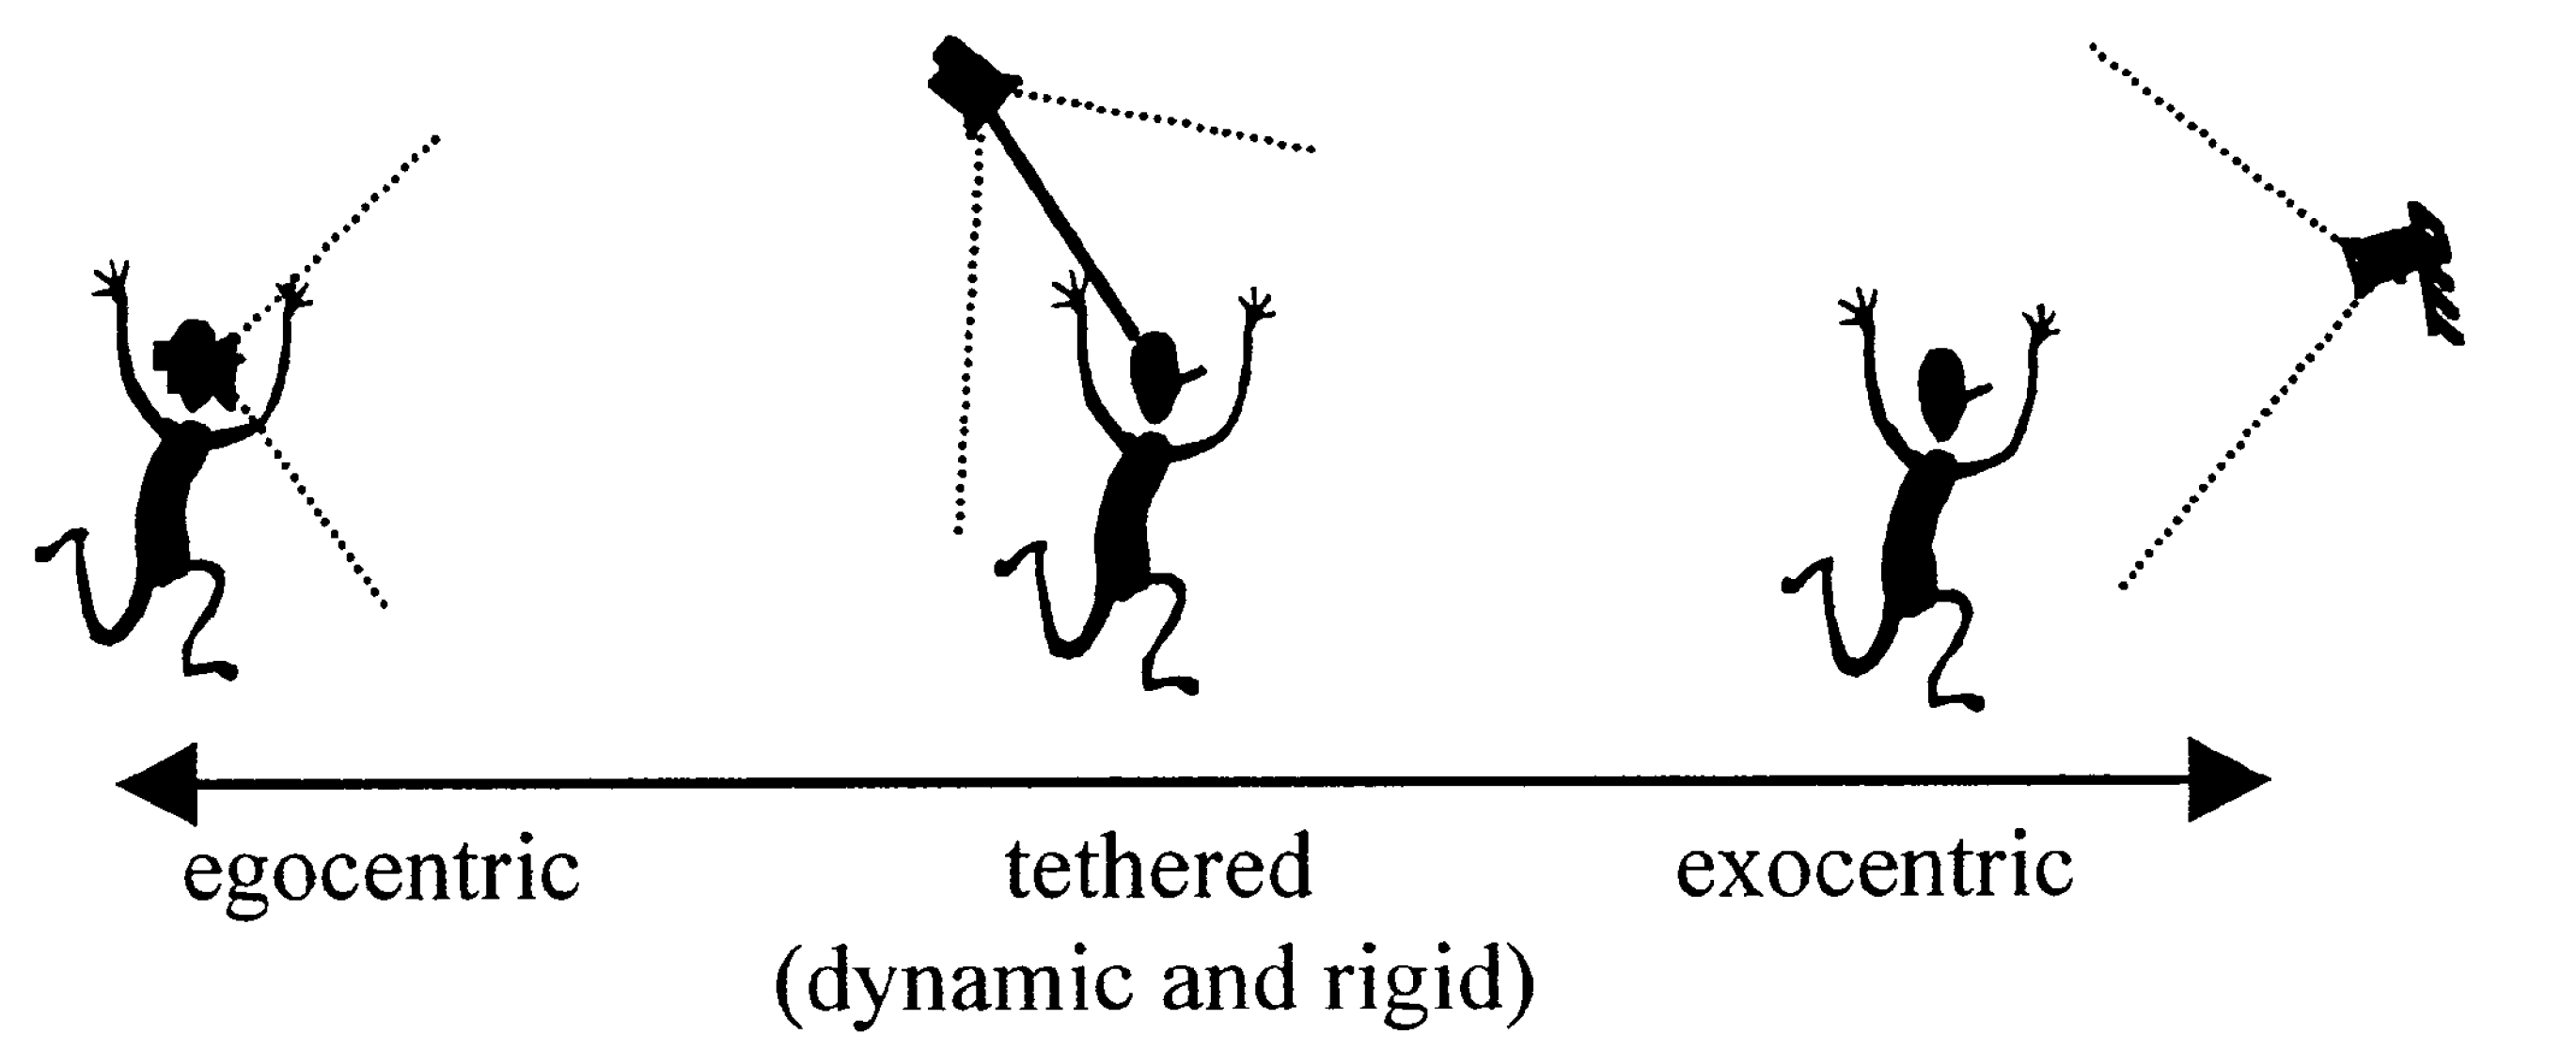
\includegraphics[width=1.0\textwidth]{img/ego_exo_continuum_bigger.PNG}
	\caption{Centricity continuum by Wang and Milgram 2001 \todo}
	\label{fig:ego-exo-cont}
\end{figure}

%welche perspektieven gibt es